\chapter{はじめに}
\section{背景}
%農業について語る。
生物が生存するために外部から栄養や水分を摂取することは必須である。
人類においても同様に栄養の摂取、つまり食事は日常的に行っている。
これはマズローの自己実現理論の最底辺に定義されているように、知能が高度に発展した人類においても栄養の摂取は生命を維持するためには必須条件である。\cite{maslow}
%参考 出典の3の本をhttps://ja.wikipedia.org/wiki/%E8%87%AA%E5%B7%B1%E5%AE%9F%E7%8F%BE%E7%90%86%E8%AB%96
\subsection{食糧事情}
%http://www.maff.go.jp/j/pr/annual/pdf/syoku_jijyou.pdf
%ほとんどこのpdfから画像とか数値とか資料ここから
食事に必要な作物は田畑で作られ、生産物は物流に乗り個人に供給されている。
この物流網はグローバル化に伴い国境を跨ぎ、海外からも供給されている。
Fig.\ref{g7hikaku}に示すのは先進主要各国の農産物の輸入額を比較したものである。
とりわけ日本は多額の農作物を海外より調達している。
これには海外と比較し生産コストや田畑に適した土地が少ない等の問題により、多くの作物が海外より輸入されることが目立つ。\cite{FoodReport}
また、Fig.\ref{suii}に示すのは日本の食糧自給率の推移をグラフで表したもので、過去20年ほどは食糧自給率が40\%程を彷徨っている。
近年では39\%にまで低下しており、Fig.\ref{g7hikaku}に示す諸外国との食糧自給率の比較においても日本の食糧自給率の低さが伺える。
\begin{figure}[b] 
    \centering
    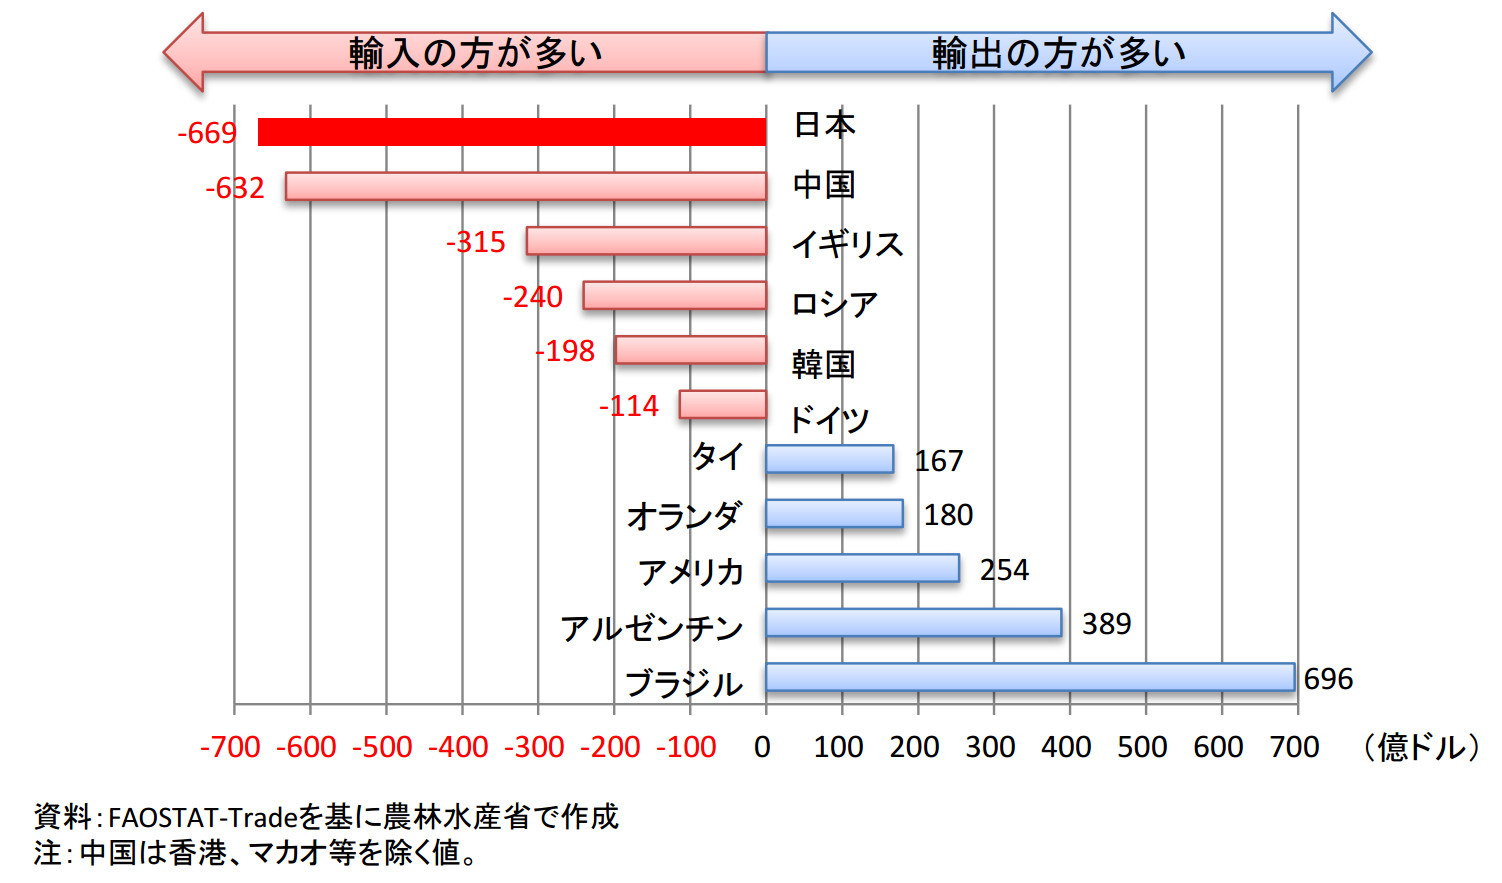
\includegraphics[width=0.5\textwidth]{image/intro/shokuryou_yunyuugaku.jpg}
    \caption{各国の農作物の輸入額-輸出額の比較(2012)} 
    \label{kingaku}
\end{figure}
\begin{figure}[b] 
    \centering
    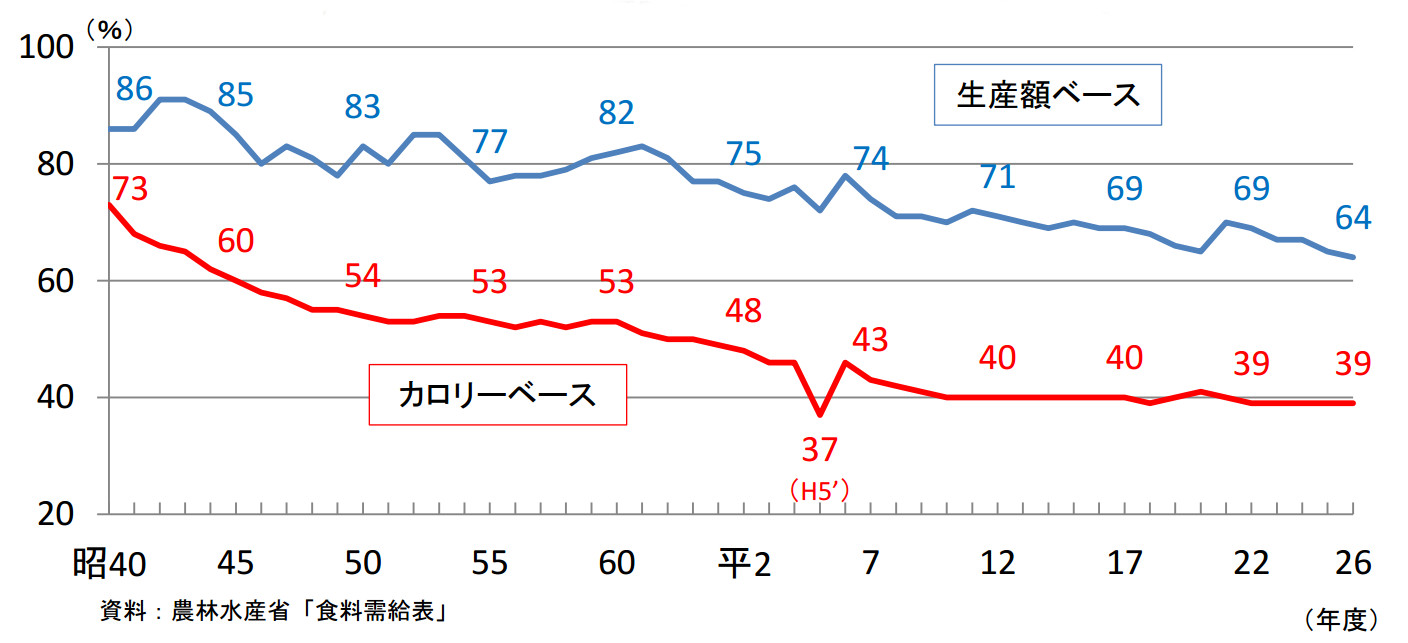
\includegraphics[width=0.5\textwidth]{image/intro/shokuryou_suii.jpg}
    \caption{食糧自給率の推移} 
    \label{suii}
\end{figure}
\begin{figure}[b] 
    \centering
    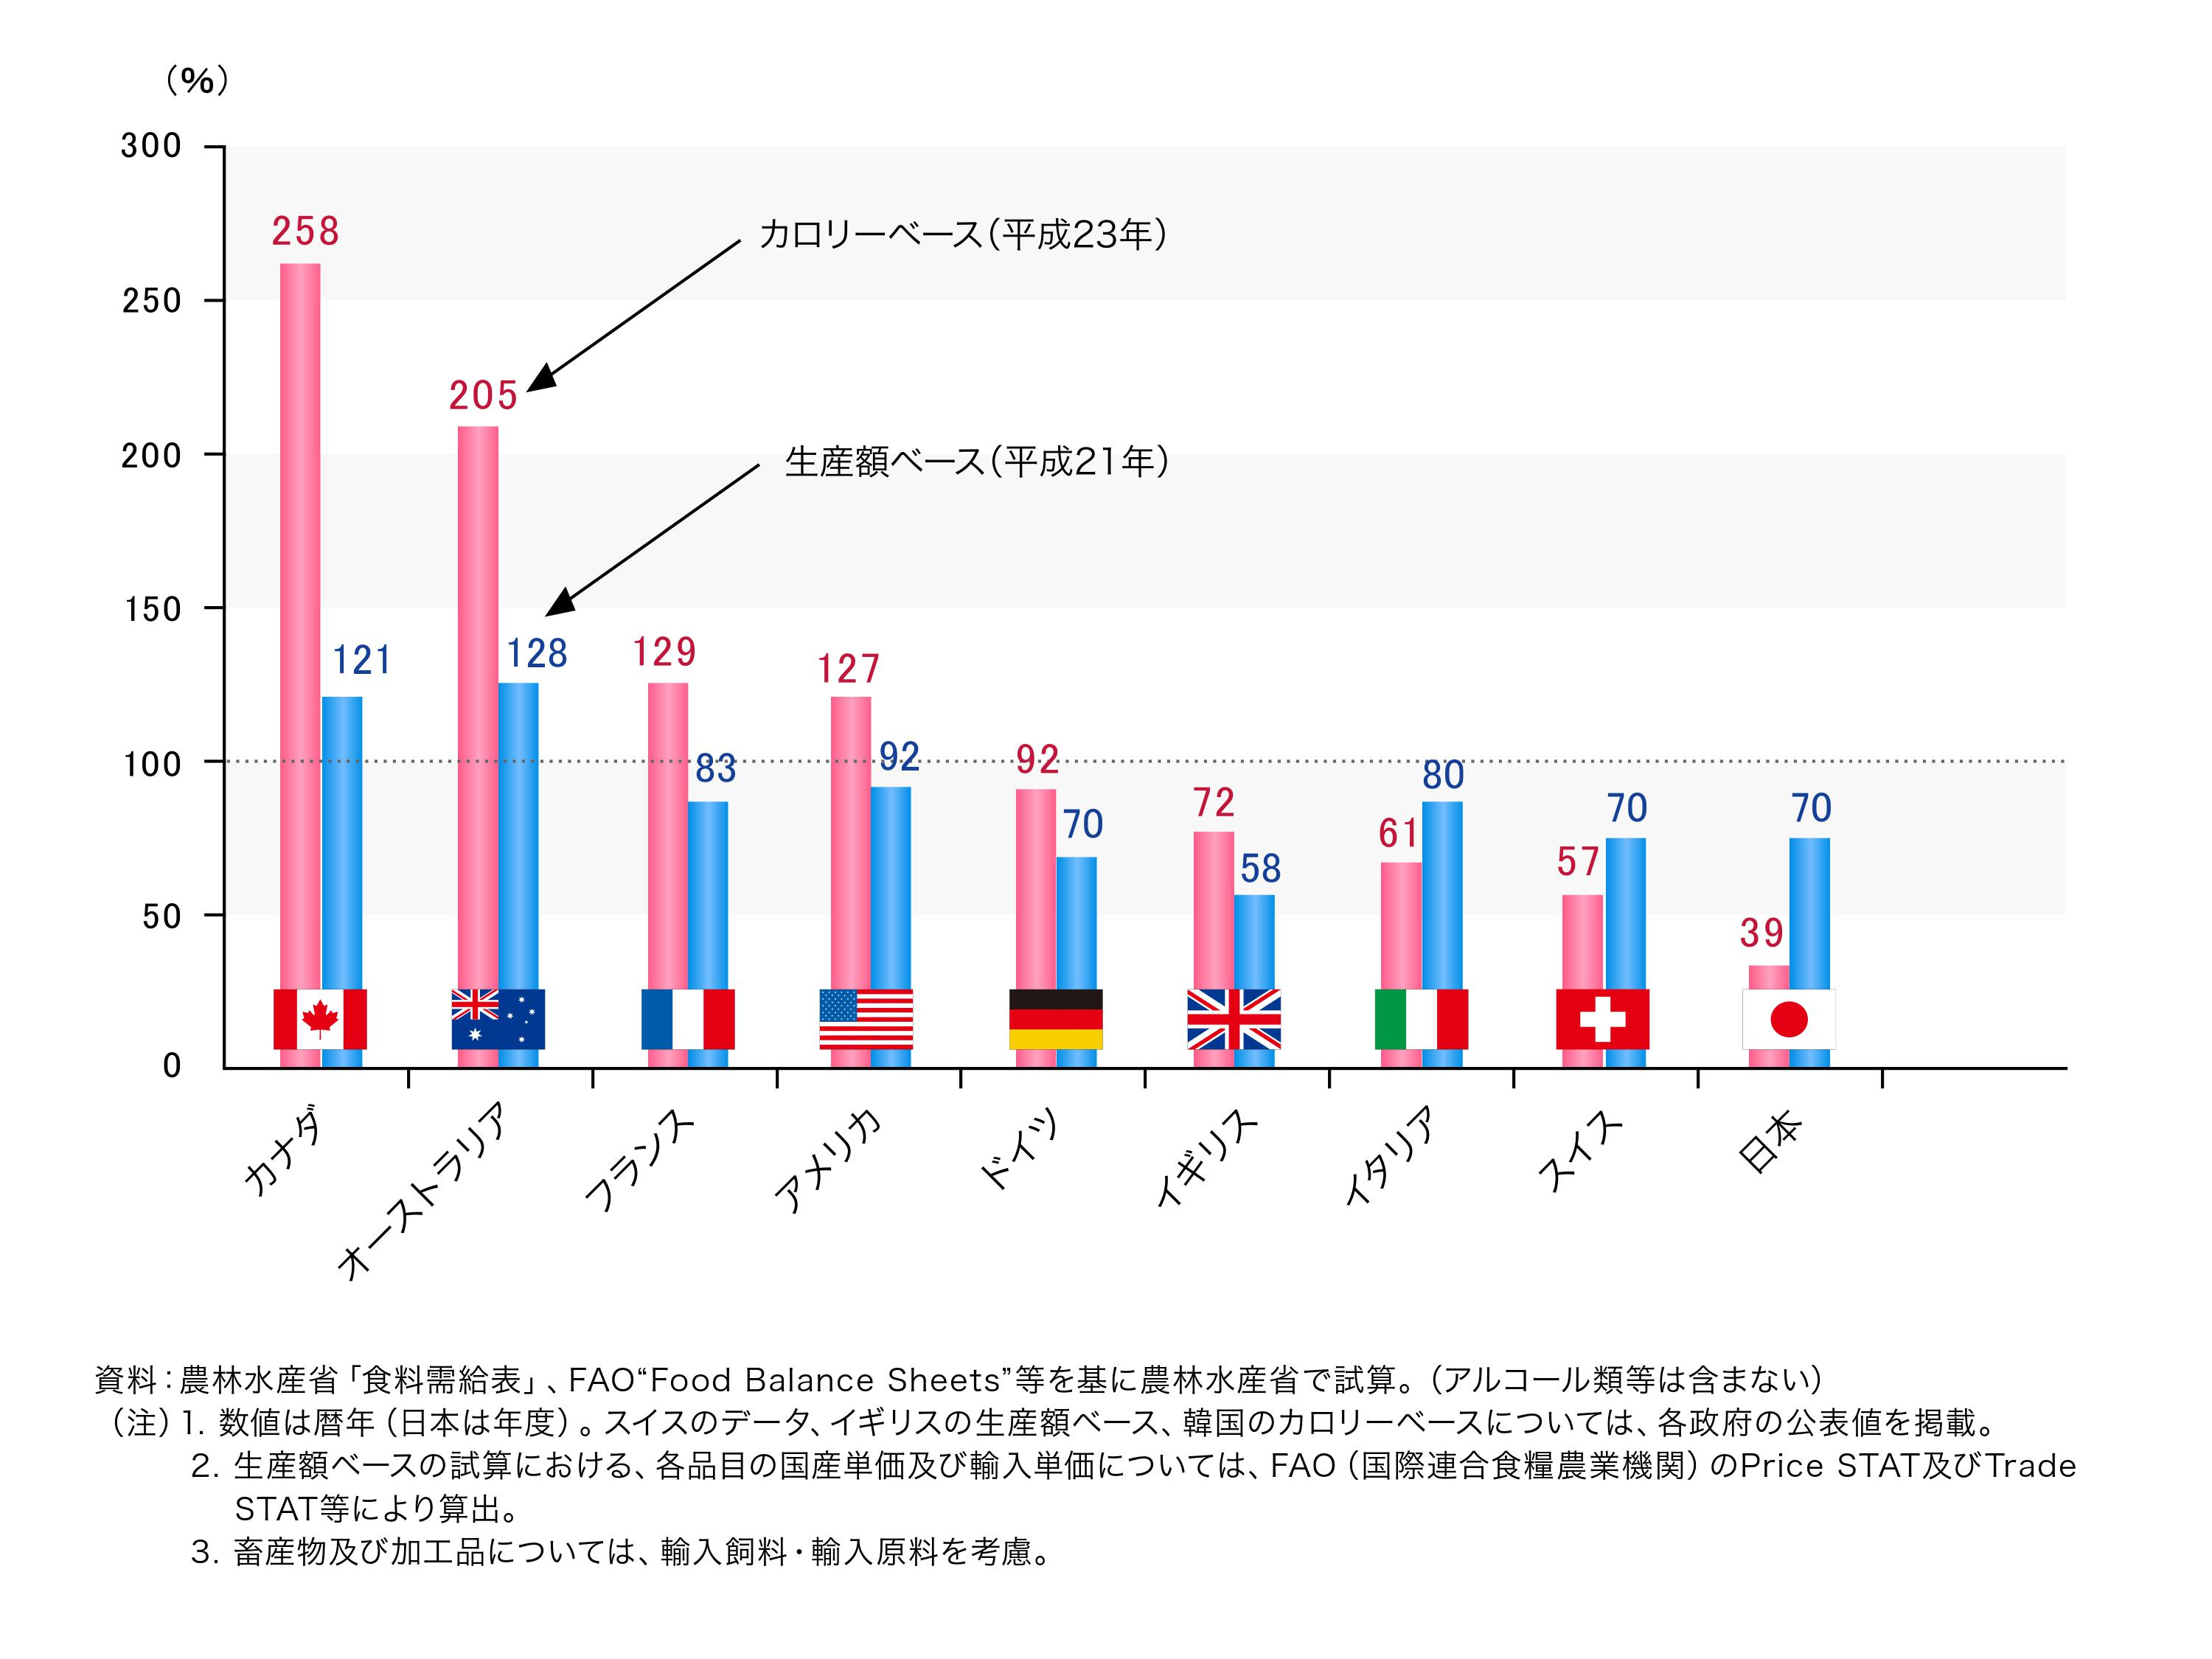
\includegraphics[width=0.5\textwidth]{image/intro/g7hikaku.jpg}
    \caption{先進主要各国の食糧自給率比較} 
    \label{g7hikaku}
\end{figure}
\subsection{食料安全保障}
食料を自国で生産できない分は必然的に海外より輸入することになる。
しかし、為替変動リスクによる調達コストの変動や、紛争による輸入の途絶により食料の調達に苦労することになる。
これらのリスクを低減するために日本では諸外国との親和を密としている。
具体的には外国為替市場介入政府\cite{boj}、開発援助 (ODA:Official Development Assistance)による技術提供や海賊がシーレーンに仕掛けた機雷撤去\cite{oda}など、一見すると国際社会貢献にも伺えるがこれらは輸入物資を安定して日本に届けるための活動である。
今日、日本が輸入に頼って安定した生活を行っているのはこれら外交による賜物である。
\subsection{リスクへの対応}
以前より前節のリスクに対する対応が注目されている。
農林水産省でのリスクへの対応では、主に次の3つが主要な柱が策定されている。\cite{FoodSafety}
\begin{description}
    \item[国内生産の増大]\mybox{}\\
        消費者ニーズに応じた国内農業の生産の拡大のため、農地や担い手の確保、農業の技術革新や食品産業との連携等により生産・供給体制の構築実現の取り組み。
    \item[輸入の安定化] \mybox{}\\
        日本は輸入相手国との良好な関係を築き、食料の安定供給の確保に資するよう国際交渉を進めている。
    \item[備蓄の確保] \mybox{}\\
        主食である米や、供給の多くが輸入に依存している小麦や飼料穀物について、一定数量の備蓄を実施している。
\end{description}
政府ではこれらの項目において、国内の農業生産の増大を図ることを基軸とした政策を掲げており、食糧自給率の底上げを念頭に農業産業の拡大化を図っている。

\subsection{間をとりもつ何か}
農業大切だよ、特に国内生産の増加。
で、私は工学的なアプローチでこれやるよって。
それを語る所。
なんて書こうか。。。

\section{従来研究}
食料生産量の増加において様々なアプローチがある。
農学、生物学、化学、工学など多岐にわたる。
本研究では工学的アプローチにより問題の解決を図る。

\subsection{農業の自動化}
%http://www.maff.go.jp/j/kanbo/kihyo03/gityo/g_smart_nougyo/pdf/cmatome.pdf
%スマート農業
農作物の生産方法で近年注目されているのが、機械やコンピュータを使った農業の自動化である。
農林水産省ではロボット技術やICT等の先端技術を活用し、超省力化や高品質生産等を可能にする新たな農業である「スマート農業」を掲げており、日本の少子高齢化や人口減少等の問題を見据えたプロジェクトである。
農業の自動化を政府が主体となり行うことで、これまで多くの研究が行われてきた。
\subsubsection{農業機械の自動化}
農業機械の自動化は着々と進んでおり、Fig.\ref{kikai_torakuta}に示す畑田を耕すトラクターやFig.\ref{kikai_konbain}の収穫を行うコンバインは自動で
\begin{figure}[b] 
    \centering
    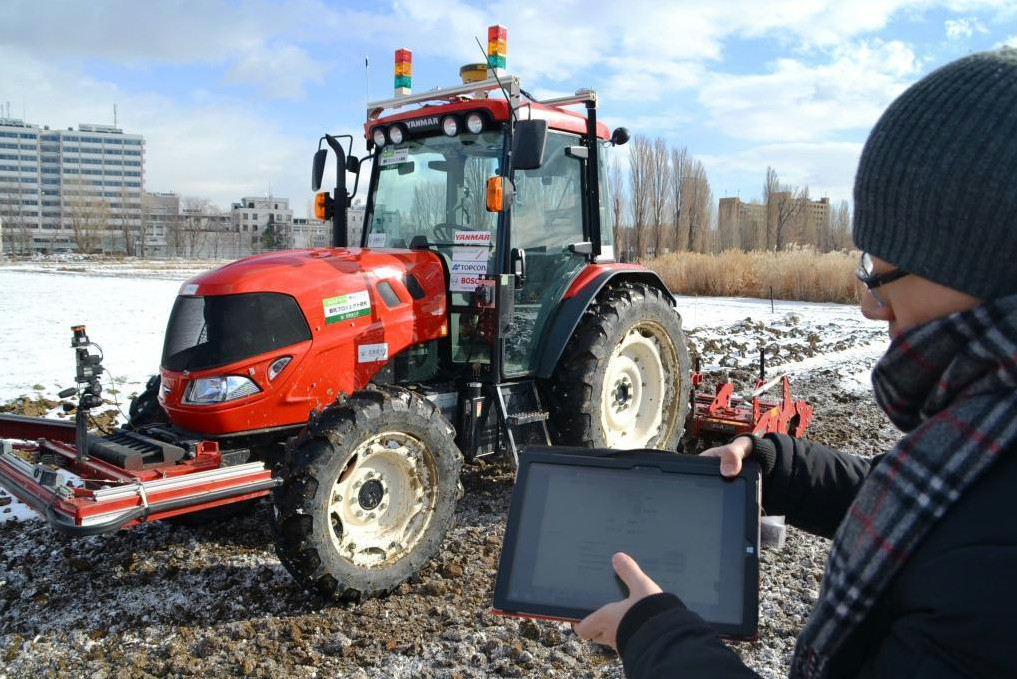
\includegraphics[width=0.5\textwidth]{image/intro/torakuta.jpg}
    \caption{農業機器の自動運転風景} 
    \label{kikai_torakuta}
\end{figure}
\begin{figure}[b] 
    \centering
    \includegraphics[width=0.5\textwidth]{image/intro/konbain.jpg}
    \caption{コンバインの自動運転風景} 
    \label{kikai_konbain}
\end{figure}
\subsubsection{農業のIoT化}
図を含めて、軽く説明する。
\subsubsection{植物工場}
図を含めて、軽く説明する。

\subsection{問題点?てきな?}
%ロボット化、機械化、流行ってるね。
%でも、結局,植物は他者に依存してるね。
%それって、危ないでしょ。気候変動で種の滅亡とかあるでしょ。あかん。
前章の研究やビジネスモデルは植物の生産性や品質の向上に寄与し、作物の話題性やブランド化による収益性の向上など商売としても前向きである。
しかし、生産方法にはいくつかの問題点が存在する。
\par はじめに技術的な問題による問題点を上げる。
1つ目に大型の生産設備を設置するにあたり、膨大な費用や時間といったコストがかかってしまう点。
2つ目に現状のロボットによる自動化工場では栽培の行える品種が限られてしまい多様性に欠けてしまう。
これらの問題にあたっては技術の進歩により解決に近づけるものとなっている。
\par 次に栽培方法そのものの問題点をあげる。現在栽培されている植物の栽培方法の多くは人ないしロボットが栽培から育成、収穫を行っている。
栽培環境においても屋外による自然任せな状況、もしくはハウス栽培など屋内において他者によって管理された環境内で栽培されている。
つまり人間が食料としとして食べている多くの植物は、他者に依存した環境下で成長し収穫されている。
これは前節で述べたように、周囲の者に依存した状況下では環境の変化に脆弱で滅亡の恐れがある。
\section{植物と動物の違い}
%自律的に行動して、他者に依存しない動物的な行動するればいいかも
%自分で光や水を求めて行動して、自分で生き抜く。雨乞いしない。
%それを実現できる物をつくる。
(植物の進化、参考文献なし)
生物は種の存続をするため進化を行ってきたとされている。
植物も長い年月をかけて現在の形になっている。
自身が動かずして養分と水分を摂取し、呼吸を行い生命活動を行っている。
これはエネルギー効率が非常に高く、植物がこれまでの進化で獲得してきた他の生物にはない最大の特徴である。
\par その一方、動物は移動能力や高い知性を持ち合わせている。
エネルギー効率こそ植物に劣るものの、環境に対して自ら行動を行えることや、集団行動を行うべくコミュニケーション能力を持ち合わせていることも動物の特徴である。
動物の行動では適切な環境への移動や、自らの生命活動に必要となる物を取得することが可能となっており、環境への適応能力が高く、人間もまた同じ能力を持ち合わせている。
植物は特定の環境下において省エネルギーに生存する一方、動物は変動する環境に対して能動的に行動を行う生存方法をとっている。
\section{研究目的}
本研究では植物において、従来獲得することのない動物的な自律した行動を行い、他者に依存しない育成システムの作製を行う。
自ら行動を行うことで本来適切でない環境においても適切な環境を探しだし、養分等を自ら獲得することで植物は自己育成を行う。
\section{論文構成}
%最後に書こう。
あとで。
